% !TEX root = ./master.tex
\section{Technique de passation du test Tomatis}
Nous allons aller plus avant sur le test d'écoute pour plus de détails et de précision sur son utilisation.

L'appareil de Tomatis, basé sur la reconnaissance des sons purs\footnote{Cf. p. 34--35, "L'oreille et le langage" Ed. Points, Science} et
permettant d'objectiver la qualité de l'écoute
 a été créé dans les années 50, comportant un générateur de fréquences
 avec
 des sons
  purs de 125 à 8000 Hz, d'octave en octave, en passant par les valeurs
1500, 3000 et 6000 Hz, et dont l'intensité peut varier de 5 en \SI{5}{\dB}, de 10 à 100 dB.
Ces derniers sont propagés par une
  transmission aérienne avec un casque, et par une propagation osseuse
  avec un vibrateur.

  L'identification de ces sons est
  signalée par la levée de la main homolatérale (droite, gauche ou
  bilatérale).
Un volume initial très faible est suivi d'une intensité
progressive jusqu'à la manifestation d'une réponse gestuelle.

Nous allons développer à l'aide de la représentation
graphique ci-dessous, (Fig 3. 3) les paramètres du\textbf{ seuil}, de la
\textbf{spatialisation}, de la \textbf{sélectivité} et de l'\textbf{au\-dio\-latérométrie}.


\begin{figure}
	\centering
	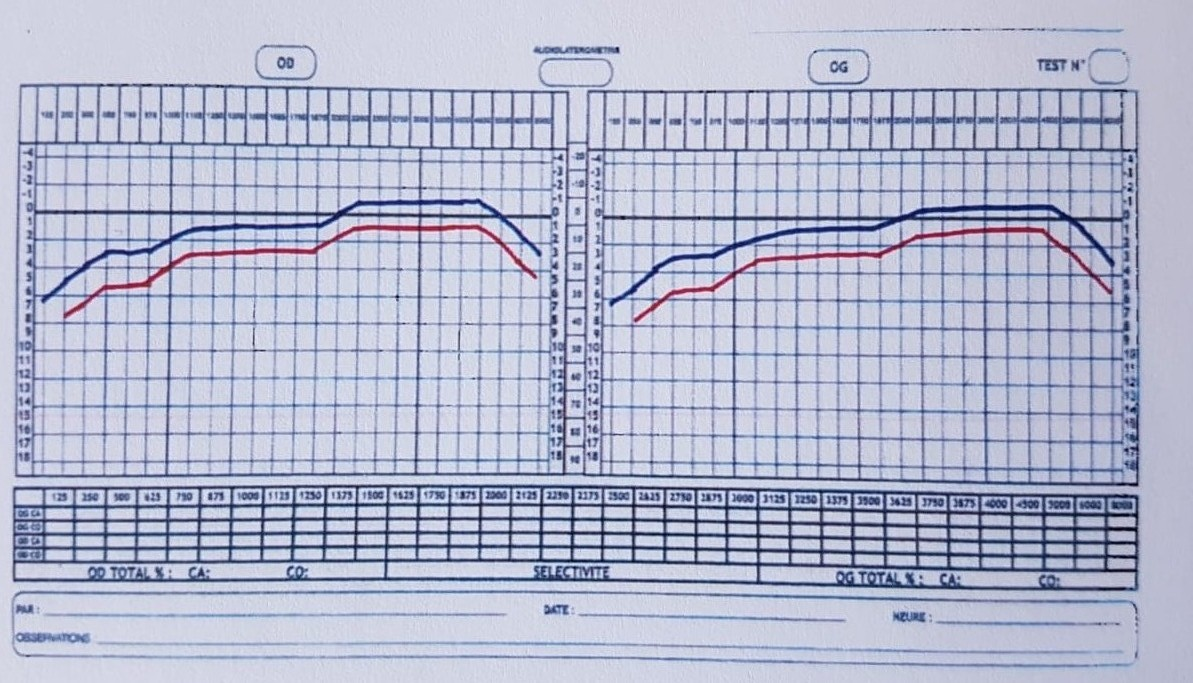
\includegraphics[width=1\linewidth]{images/courbeideale.jpg}
	\caption{Diagrammes des courbes relatives à l'oreille droite et
          gauche; tracé bleu: c. aérienne; tracé rouge: c.
          osseuse, (Copyrights Tomatis Développement S.A.  2014) }
	\label{fig:courbeideale}
\end{figure}




\subsection{Identification des seuils auditifs individuels}

Cette \textbf{détection}, destinée à relever les deux profils d'écoute
en vue d'une application thérapeutique,
s'effectue, d'une part, à l'aide d'une
conduction aérienne par \textbf{écouteurs}, où l'oreille interne
informe le nerf auditif,  et d'autre part, à l'aide
d'une conduction osseuse par\textbf{ vibrateur}, excitant le crâne au
niveau de l'
\textit{os mastoïde} transmettant à son tour à  la voie nerveuse
auditive.

\subsection{Représentation graphique}

Parmi les quelques éléments différentiels
apparaissant par la suite dans les observations cliniques, il est utile de retenir
que le \textbf{seuil d'écoute} est représenté par un point, résultant entre la
fréquence (abcisse) --spectre couvrant 20
fréquences (de 125 à 8000 Hz)--   et le volume
(ordonnée) dont chaque carré représente une différence de \SI{5}{\dB} en
volume, partant de dB de $-20$ à 90 dB.


Les points reliés dessinent deux courbes caractéristiques, (aérienne
et osseuse), permettant de relever les paramètres d'harmonie ou
          d'équilibre, ceci
 	en comparaison avec la courbe idéale : on parlera
        d'équilibre ou de
 	déséquilibre, d'harmonie ou de dysharmonie.

        \begin{enumerate}

  \item   Les seuils d'écoute sont reconnaissables par des points au niveau de
          chaque fréquence émise et selon le volume entendu par le
          patient. Les points reliés créent les deux courbes.
 	\item Le son : son pur en 20 fréquences différentes, de 125 à 8000 Hz.
 	\item Le volume: dB de $-20$ à 90; un carré sur le graphique représente une différence de \SI{5}{\dB} en
 		volume
 	\item La courbe: est le résultat des points reliés des seuils
          d'écoute; ils
          dessinent deux courbes caractéristiques, l'une aérienne et l'autre osseuse.
\item L'équilibre/déséquilibre graphique s'observe
        -entre les deux oreilles, l'oreille droite et l'oreille gauche
        et
        -entre les deux courbes aériennes et osseuses, dont les
        croisements, les pics ou les échancrures notifient
        l'écart en
        qualifiant l'écoute d'harmonieuse ou de
        déséquilibrée.
      \end{enumerate}

 En  conséquence,  s'il y a une modification
          graphique des courbes, elle
          permettra de constater s'il y a \textbf{une transformation de l'écoute}
          pour répondre à la première hypothèse et aussi d'évaluer cette transformation de l'écoute pré -- et
          post -- thérapie.




Soulignons que Tomatis a volontairement décalé les étalonnages des deux courbes (aérienne et osseuse) pour pouvoir distinguer les différentes réponses et interpréter
	les \textbf{distorsions}. Lorsque l'écoute est harmonieuse, les
	courbes aérienne et osseuse se confondent mais pour l'analyse des
	résultats, on a déterminé des courbes parallèles, la courbe aérienne
	devant être au dessus de la courbe osseuse.


\begin{figure}
	\centering
	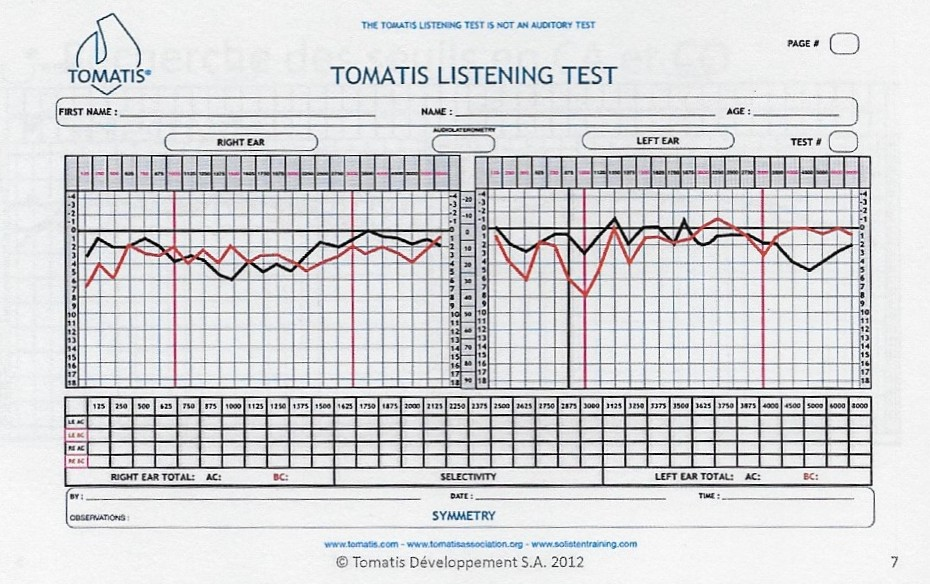
\includegraphics[width=1\linewidth]{images/tomatisListeningTest.jpg}
	\caption[Test d'écoute]{Test
          d'écoute dit asymétrique, avec o.d. + o.g. incluant, en bas, le test de sélectivité}
	\label{fig:tomatislisteningtest}
\end{figure}



Nous énumèrerons brièvement les
différentes techniques d'observation telles la
\textbf{spatialisation, la
sélectivité et l'audiolatérométrie}, mentionnées car importantes.
 Il serait intéressant d'englober ici tous ces paramètres mais
  l'objectif de notre travail serait largement dépassé.
Vu sous l'unique angle de l'observation de la transformation de l'écoute, nous
donnerons ici la priorité à la comparaison graphique
de la courbe aérienne et osseuse. Appuyé par les résultats
% quantitatifs
des \textbf{seuils auditifs}
\footnote{Nous nous référons à
  l'étude effectuée par le CNRS de Montpellier,\autocite{affectiveDisorders}.},
le nombre de \textbf{croisements }sera
également quantifié.

Nous nous permettrons d'élargir, en
complément d'information, l'exemple d'un test d'écoute d'un patient en détaillant l'impact
des\textbf{ trois zones} et leur corrélation psychique.



\subsection{La spatialisation}




En relevant les seuils, on assiste à la capacité
d'\textbf{identification} et de \textbf{localisation} de la
\textbf{source sonore} comportant parfois des confusions et/ou des inversions
latérales.

La \textbf{spatialisation}
indique le degré d'élaboration de la latéralité auditive,
et elle fournit des repères sur la façon dont le cortex intègre les informations
par les faisceaux homo et hétéro -- latéraux fonctionnellement différenciés.
Selon Tomatis, les erreurs de spatialisation peuvent refléter cette confusion des informations et traduire une latence/
incertitude de localisation de la provenance du son, difficulté due à une mauvaise coordination.
\subsection{La sélectivité}


  La \textbf{sélectivité }s'assimile  à  la CAT, capacité d'analyse tonale, \textquote{faculté que possède une oreille de percevoir
une variation de fréquences à l'intérieur d'un spectre sonore, et
de situer le sens de cette variation}\autocite{tomatis:loreille} dont
le but est de déceler l'ouverture ou la fermeture de cette
caractéristique auditive.

La sélectivité permet de donner des informations sur la
qualité d'écoute. Elle touche aux aspects  linguistiques (conscience
phonémique), cognitifs (fonctions exécutives) et émotionnels (action
efférente, présence d'anxiété).


Le langage étant lui-même constitué de milliers de phonèmes, Tomatis reconnaît les possibilités auditives du patient si celui-ci  distingue au minimum la différence d'un son ``pur" \footnote{Cf. Annexe A. 1. } d'une octave à l'autre.


\subsection{ L'audiolatérométrie}

Grâce à l'\textbf{audiolatérométrie}, on définit  la latéralité droite ou gauche du patient. La dominance
de l'oreille droite comme oreille directrice doit être manifeste car
selon ses travaux, il y a une différenciation fonctionnelle
physiologique due à la longueur des nerfs récurrents.
Si le cerveau préfère prendre l'oreille droite comme
``directrice'', c'est que le trajet emprunté par l'oreille droite au cerveau est plus
court; ainsi les informations circulent plus rapidement jusqu'à l'hémisphère gauche.

          \paragraph{\textbf{Par conséquent,}}après la passation du test d\textquoteright écoute, nous nous
trouvons en présence de deux grilles contenant chacune deux courbes,
en général, de deux couleurs différentes complétées par l'indication
des inversions ou confusions de sons, par des données sur la sélectivité
et en même temps par des chiffres qui correspondent à l'épreuve d'audiolatérométrie.
Les résultats du test permettront de faire une comparaison avec la
courbe dénommée idéale\footnote{Cf.\textit{ Caruso } Ch. 3. 1.)}.


\subsection{Les trois zones du test d'écoute }
Sur le graphique du test, les fréquences observées vont être partagées en
trois, permettant la mise en évidence de différentes zones à l\textquoteright intérieur
de chaque diagramme. Les fréquences se répartissent des
graves aux aigues, de la façon suivante :
\begin{itemize}
\item Zone 1 : de 125 à 1000 Hz : les graves, la zone vestibulaire
\item Zone 2 : de 1000 à 3000 Hz : les mediums, la zone du langage
\item Zone 3 : de 3000 à 8000 Hz : les aigus, zone cochléaire
\end{itemize}
Ces différentes bandes de fréquences sonores nous donneront des éléments
d'interprétation.
Nous nous appuyons ici sur les affirmations expérimentales de Tomatis.
%\footnote{ Ces données interprétatives sont fiables, confirmées par
 % les recherches de Tomatis dans le domaine
  %empirique.}

\subsection {Analyse et interprétation du test}


De manière générale, l'interprétation du test insiste sur le relevé graphique
des
courbes et accorde des
significations différentes aux zones spectrales.
On considère d'abord l'\textbf{allure }générale des courbes, leur
\textbf{dessin} et la \textbf{forme}, l' \textbf{équilibre}, la \textbf{symétrie}  :
puis on estime
leur\textbf{ rapport} entre eux -- entre la courbe aérienne (CA) -- et la courbe osseuse (CO),
pour chaque oreille ainsi que le rapport entre CA et CO d\textquoteright une
oreille à l'autre. Si ce rapport est correct, CA est placée au-dessus
de CO sur la grille.

Les courbes donnent des informations selon leur ascendance, leur
continuité et leur similarité oreille droite/ oreille gauche.

Chacune  véhicule des informations spécifiques
sur la posture d'écoute du sujet :
\begin{itemize}
\item La conduction aérienne : traduit la vie sociale, la manière de communiquer
et de s'extérioriser.
\item La conduction osseuse : traduit la vie intérieure, mode de fonctionnement
organique, d'une façon générale : liée aux tensions. C'est la courbe
de l\textquoteright auto-écoute, de l\textquoteright auto-contrôle,
de l'écoute intérieure.
\end{itemize}

Une courbe est définie comme \textbf{harmonieuse}\footnote{Cf. Ch. 1. 2. / 3.1.}
si elle ne comporte pas de
pics, de scotomes
qui laisseraient
supposer l'existence de nombreuse tensions.
Situées en CO, ce sont des tensions internes non exprimées : attitude
calme mais très tendue intérieurement.
Situées en CA, ce sont des tensions réelles et exprimées au quotidien
: soit somatisées, soit verbalisées ou soit manifestées sur le plan
affectif (pleurs).



\subparagraph{Interprétation des trois zones du test d'écoute : }
\begin{itemize}
\item Zone 1 : de 125 à 1000 Hz : les graves, la zone vestibulaire, élaboration
du schéma corporel, des repères temporo-spatiaux, adresse motrice,
esprit pratique.
\item Zone 2 : de 1000 à 3000 Hz : les mediums, la zone du langage, de la
  verbalisation, compréhension, (Wernicke),
 mémorisation (Papez), de l'intégration des lois/
 des règles, esprit analytique.
 %lobes frontaux,
\item Zone 3 : de 3000 à 8000 Hz : les aigus, zone cochléaire, de l'énergie,
  de l'imagination, de l'expression, motivation.
  fonctions de survie, pulsion à l'état primitif, cortex
 hautement spécialisé), esprit synthétique.
\end{itemize}

Les trois zones de fréquences du test d'écoute correspondent à des
caractéristiques précises ; et, avec l'allure des courbes, on doit
tenir compte de leurs particularités.


\textbf{Remarque:} dans le travail qui va suivre, l'allure générale des courbes, le relevé quantitatif des
  croisements et des seuils auditifs seront notre priorité pour
  extraire nos résultats à partir de ces tests.

Nous disposons à présent d'une somme suffisante de renseignements pour
aborder le chapitre suivant consacré à l'étude clinique et
l'illustrer par des exemples.
La simplicité de
passation du test d'écoute est remarquable -- ce qui le rend d'autant
plus pertinent dans le cadre du travail présent -- et les réponses gestuelles
 donnent des indices de réception %évitant toute confusion
quelle que soit la langue utilisée,\textbf{ procédé non-verbal
spécifiquement axé sur le son.}



\begin{figure}
	\centering
	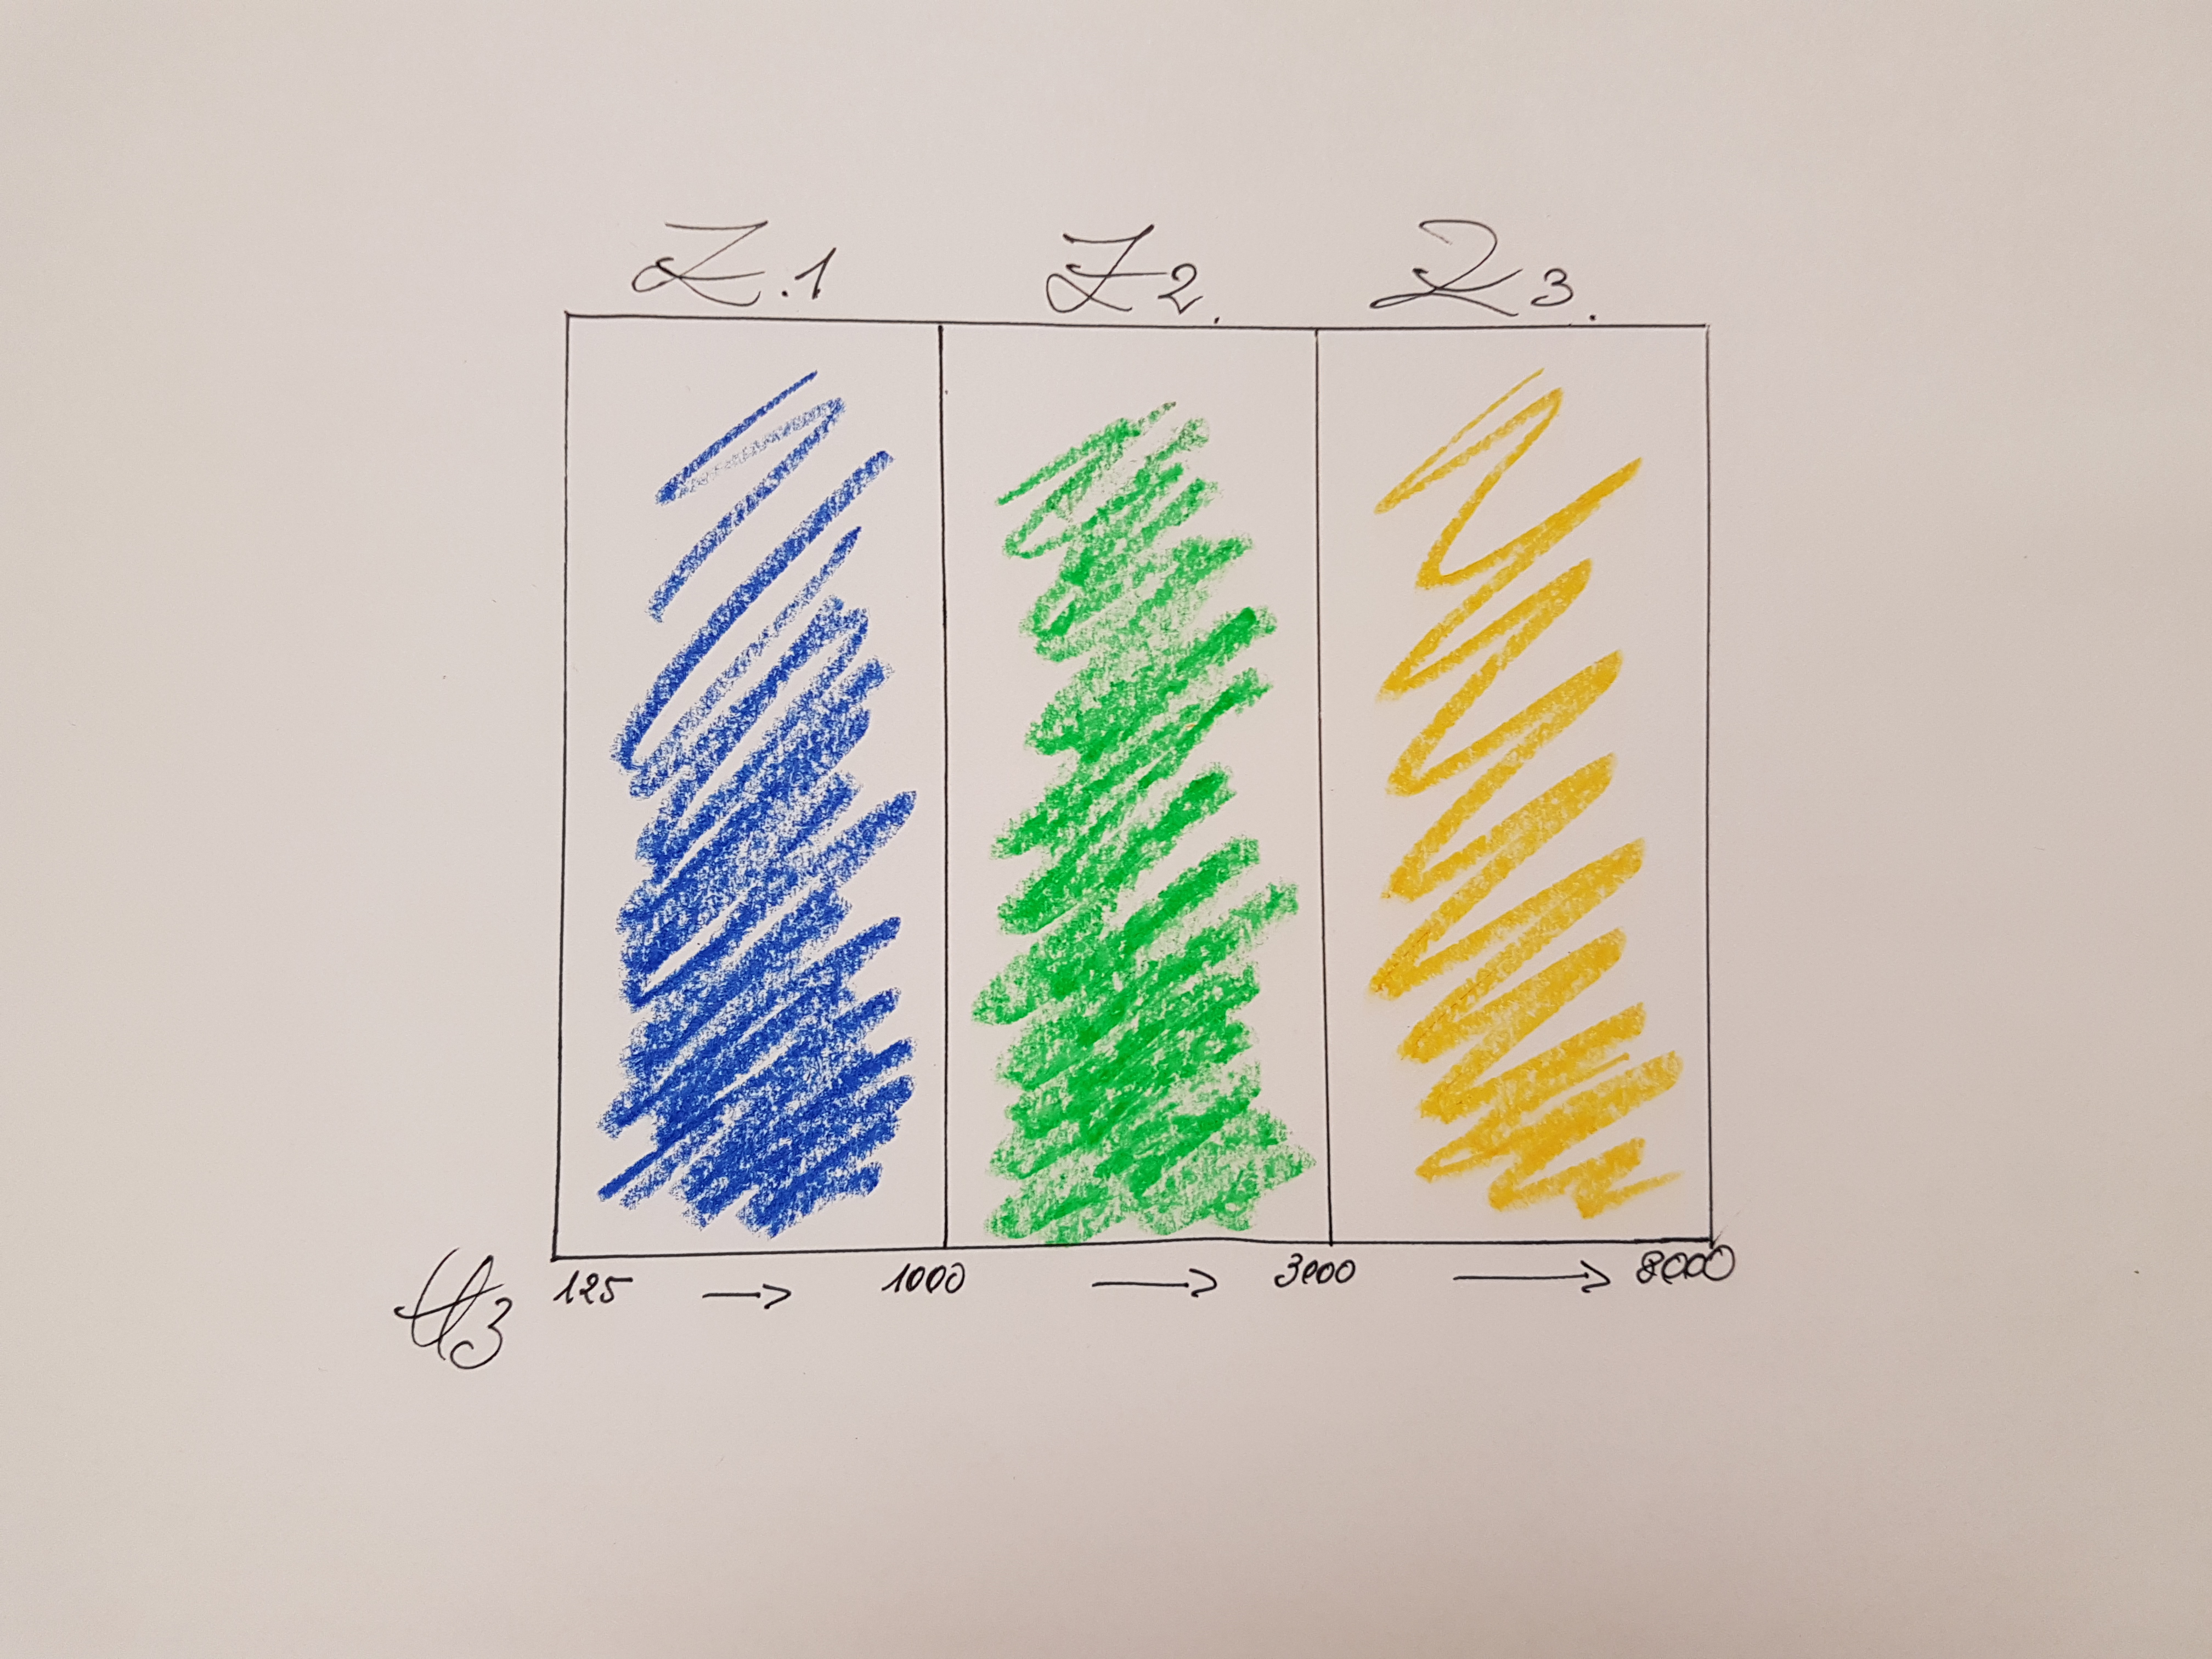
\includegraphics[width=1\linewidth]{images/les3zones.jpg}
	\caption[Les 3 zones]{Les 3 zones}
	\label{3zones}
\end{figure}
